\documentclass[tikz,border=2pt]{standalone}
\usetikzlibrary{arrows.meta}
\tikzset{sym/.style={line width=2pt, draw=black, line cap=round, line join=round}}
\begin{document}
% Lesson 1 What is science: a magnifying glass over a question mark

\begin{tikzpicture}
  \draw[sym] (1.6,1.9) circle (1.3);
  \draw[black, line width=5pt, line cap=round] (2.55,0.95) -- (3.7,-0.2);
  \node[font=\fontsize{60}{60}\selectfont\bfseries\sffamily] at (1.6,1.9) {?};
  \draw[sym] (0.65,3.0) arc[start angle=135, end angle=165, radius=1.3];
\end{tikzpicture}
% Lesson 4 The scientific method: a loop of five steps
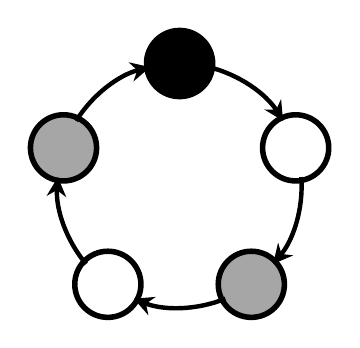
\begin{tikzpicture}
  \foreach \a/\f in {90/black, 18/white, -54/black!35, -126/white, 162/black!35}{
    \draw[sym, fill=\f] (\a:1.55) circle (0.42);}
  \foreach \a in {90,18,-54,-126,162}{
    \draw[black, line width=1.6pt, -{Stealth[length=7pt,width=7pt]}] (\a-14:1.55) arc[start angle=\a-14, end angle=\a-58, radius=1.55];}
\end{tikzpicture}
% Lesson 5 Safety: safety glasses and a hazard triangle
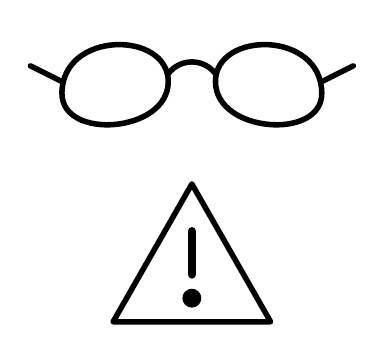
\begin{tikzpicture}
  \draw[sym] (0,0.8) .. controls (0,1.6) and (1.35,1.6) .. (1.35,0.95) .. controls (1.35,0.3) and (0,0.2) .. (0,0.8);
  \draw[sym] (3.3,0.8) .. controls (3.3,1.6) and (1.95,1.6) .. (1.95,0.95) .. controls (1.95,0.3) and (3.3,0.2) .. (3.3,0.8);
  \draw[sym] (1.35,1.05) .. controls (1.5,1.25) and (1.8,1.25) .. (1.95,1.05);
  \draw[sym] (0,0.95) -- (-0.4,1.15) (3.3,0.95) -- (3.7,1.15);
  \draw[sym, fill=white] (0.65,-2.1) -- (2.65,-2.1) -- (1.65,-0.35) -- cycle;
  \draw[black, line width=3pt, line cap=round] (1.65,-0.95) -- (1.65,-1.5);
  \fill (1.65,-1.8) circle (0.12);
\end{tikzpicture}
\end{document}
